% Don't like 10pt? Try 11pt or 12pt
\documentclass[9pt]{extreport}
%\usepackage[scaled]{helvet}
\renewcommand\familydefault{\sfdefault} 
\usepackage[T1]{fontenc}
%\usepackage{lmodern}
%\usepackage{mathpazo}
\usepackage{kpfonts}
 %\usepackage{mathptmx}
%\setmainfont{uarial}
% This is a helpful package that puts math inside length specifications
\usepackage{calc}
\usepackage[colorlinks,urlcolor=blue]{hyperref}
%\usepackage[pdftex]{graphicx}
\usepackage{graphicx}
\usepackage{wrapfig}
% Simpler bibsection for CV sections
% (thanks to natbib for inspiration)
\makeatletter
\newlength{\bibhang}
\setlength{\bibhang}{1em}
\newlength{\bibsep}
 {\@listi \global\bibsep\itemsep \global\advance\bibsep by\parsep}
\newenvironment{bibsection}%
        {\vspace{-\baselineskip}\begin{list}{}{%
       \setlength{\leftmargin}{\bibhang}%
       \setlength{\itemindent}{-\leftmargin}%
       \setlength{\itemsep}{\bibsep}%
       \setlength{\parsep}{\z@}%
        \setlength{\partopsep}{0pt}%
        \setlength{\topsep}{0pt}}}
        {\end{list}\vspace{-.6\baselineskip}}
\makeatother

% Layout: Puts the section titles on left side of page
\reversemarginpar

%% Use these lines for letter-sized paper
\usepackage[paper=letterpaper,
            %includefoot, % Uncomment to put page number above margin
            marginparwidth=1in,     % Length of section titles
            marginparsep=.09in,       % Space between titles and text
            margin=.6in,               % 1 inch margins
            includemp]{geometry}

%% More layout: Get rid of indenting throughout entire document
\setlength{\parindent}{0in}

%% This gives us fun enumeration environments. compactitem will be nice.
\usepackage{paralist}

\usepackage{fancyhdr,lastpage}
\pagestyle{fancy}
\pagestyle{empty}      % Uncomment this to get rid of page numbers
\fancyhf{}\renewcommand{\headrulewidth}{0pt}
\fancyfootoffset{\marginparsep+\marginparwidth}
\newlength{\footpageshift}
\setlength{\footpageshift}
          {0.5\textwidth+0.5\marginparsep+0.5\marginparwidth-2in}
\lfoot{\hspace{\footpageshift}%
       \parbox{4in}{\, \hfill %
                    \arabic{page} of \protect\pageref*{LastPage} % +LP
%                    \arabic{page}                               % -LP
                    \hfill \,}}

% Finally, give us PDF bookmarks
\usepackage{color,hyperref}
\definecolor{darkblue}{rgb}{0.0,0.0,0.3}
\hypersetup{colorlinks,breaklinks,
            linkcolor=darkblue,urlcolor=darkblue,
            anchorcolor=darkblue,citecolor=darkblue}

% The title (name) with a horizontal rule under it
%
% Usage: \makeheading{name}
%
% Place at top of document. It should be the first thing.
\newcommand{\makeheading}[1]%
        {\hspace*{-\marginparsep minus \marginparwidth}%
         \begin{minipage}[t]{\textwidth+\marginparwidth+\marginparsep}%
                {\Large \bfseries #1}\\[-0.15\baselineskip]%
                 \rule{\columnwidth}{1pt}%
         \end{minipage}}

\newcommand{\makechapter}[1]%
        {\hspace*{-\marginparsep minus \marginparwidth}%
         \phantomsection\addcontentsline{toc}{section}{#1}%
         \begin{minipage}[t]{\textwidth+\marginparwidth+\marginparsep}%
                %\vspace %
                \vspace{3 mm}
                {\large \bfseries #1}%\\[-0.15\baselineskip]%
                %\vspace{-.4\baselineskip}
                %\rule{\columnwidth}{1pt}%
         \end{minipage}}

% The section headings
%
% Usage: \section{section name}
%
% Follow this section IMMEDIATELY with the first line of the section
% text. Do not put whitespace in between. That is, do this:
%
%       \section{My Information}
%       Here is my information.
%
% and NOT this:
%
%       \section{My Information}
%
%       Here is my information.
%
% Otherwise the top of the section header will not line up with the top
% of the section. Of course, using a single comment character (%) on
% empty lines allows for the function of the first example with the
% readability of the second example.
\renewcommand{\section}[2]%
        {\pagebreak[2]\vspace{0.8\baselineskip}%
         %\phantomsection\addcontentsline{toc}{section}{#1}%
         \hspace{0in}%
         \marginpar{
         \raggedright \emph{#1}}#2}

\newcommand{\ssection}[2]%
        {\pagebreak[2]\vspace{0.3\baselineskip}%
         \hspace{0in}%
         \marginpar{
         \raggedright \emph{#1}}#2}


% An itemize-style list with lots of space between items
\newenvironment{outerlist}[1][\enskip\textbullet]%
        {\begin{itemize}[#1]}{\end{itemize}%
         \vspace{-.4\baselineskip}}

% An environment IDENTICAL to outerlist that has better pre-list spacing
% when used as the first thing in a \section
\newenvironment{lonelist}[1][\enskip\textbullet]%
        {\vspace{-\baselineskip}\begin{list}{#1}{%
        \setlength{\partopsep}{0pt}%
        \setlength{\topsep}{0pt}}}
        {\end{list}\vspace{-.4\baselineskip}}

% An itemize-style list with little space between items
\newenvironment{innerlist}[1][\enskip\textbullet]%
        {\vspace{0.2\baselineskip}\begin{compactitem}[#1]}{\end{compactitem}}

% An environment IDENTICAL to innerlist that has better pre-list spacing
% when used as the first thing in a \section
\newenvironment{loneinnerlist}[1][\enskip\textbullet]%
        {\vspace{-\baselineskip}\begin{compactitem}[#1]}
        {\end{compactitem}\vspace{-.4\baselineskip}}

% To add some paragraph space between lines.
% This also tells LaTeX to preferably break a page on one of these gaps
% if there is a needed pagebreak nearby.
\newcommand{\blankline}{\quad\pagebreak[2]}

% Uses hyperref to link DOI
%\newcommand\doilink[1]{\href{http://dx.doi.org/#1}{#1}}
%\newcommand\doi[1]{doi:\doilink{#1}}


%%%%%%%%%%%%%%%%%%%%%%%% End Helper Commands %%%%%%%%%%%%%%%%%%%%%%%%%%%

%%%%%%%%%%%%%%%%%%%%%%%%% Begin CV Document %%%%%%%%%%%%%%%%%%%%%%%%%%%%

\begin{document}
\makeheading{{\sc \LARGE Publications} \hfill Duc Tam Hoang}
\begin{wrapfigure}[0]{r}{2.5cm}
\begin{center}
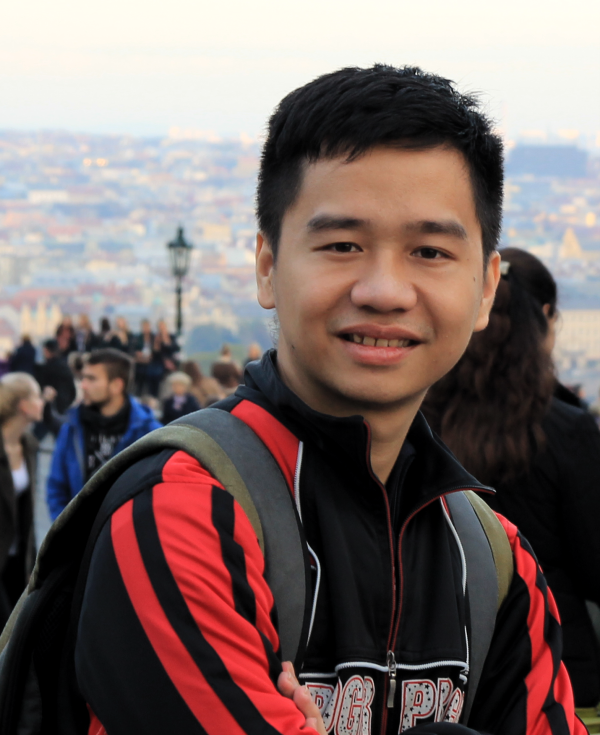
\includegraphics[width=2.5cm]{tamhd_2.png}
\end{center}
\end{wrapfigure}

\makechapter{Contact Information}

\newlength{\rcollength}\setlength{\rcollength}{1.85in}%
%
\section{Name} 
\textbf{Duc Tam Hoang} (or simply \textbf{Tam Hoang})

%\href{http://mff.cuni.cz/}{Mathematics and Physics Faculty, Charles University in Prague}
Computational Linguistics Lab, National University of Singapore

\ssection{Address}
%527, Koleje Otava, Chemick\'a 954, Praha 4, Prague
\# 05-407, Block 117, Lorong 1 Toa Payoh, 310117, Singapore

\ssection{Email}
%\href{mailto:tamhd1990@gmail.com}{tamhd1990@gmail.com}
\href{mailto:hoangdt@comp.nus.edu.sg}{hoangdt@comp.nus.edu.sg}

\ssection{Mobile}
+65 90548590

\ssection{Skype}
tamhd1990


\makechapter{Publications}
Over the years, I have worked on a number of topics. 
As a results, I have a few publications that I would like to present. 
The list contains both published paper and the upcoming papers.

\blankline

\textbf{Grammatical Error Correction}:
I have worked on Grammatical Error Correction since I became a research assistant at the National University of Singapore. It has been 6 months and we have submitted two papers to IJCAI 2016 and ACL 2016. 

\begin{enumerate}
	
	\item[4.] \underline{Duc Tam Hoang}, Ond\v{r}ej Bojar. \textbf{TmTriangulate: A Tool for Phrase-Table Triangulation}. The Prague Bulletin of Mathematical Linguistics, 2015.
	
\end{enumerate}

\blankline

\textbf{Statistical Machine Translation}:
I spent one year doing the master thesis in Statistical Machine Translation. 



\begin{enumerate}

\item[4.] \underline{Duc Tam Hoang}, Ond\v{r}ej Bojar. \textbf{TmTriangulate: A Tool for Phrase-Table Triangulation}. The Prague Bulletin of Mathematical Linguistics, 2015.

\end{enumerate}

\blankline

\textbf{Question Answering}
\begin{enumerate}

\item[3.] Tung Xuan Vu, Minh Le Nguyen, \underline{Duc Tam Hoang}. \textbf{Semantic Parsing for Vietnamese Question Answering System}. The 7th international conference on Knowledge and Systems Engineering, Vietnam, 2015.

\item[2.] \underline{Duc Tam Hoang}, Minh Le Nguyen, Son Bao Pham. \textbf{L2S: Transforming natural language questions to SQL queries}. The 7th international conference on Knowledge and Systems Engineering, Vietnam, 2015.

\item[1.] Dat Tien Nguyen, \underline{Duc Tam Hoang}, Son Bao Pham. \textbf{A Vietnamese Natural Language Interface to Database}. Sixth IEEE International Conference on Semantic Computing, Italy, 2012.
\end{enumerate}

\textbf{Others}
\begin{enumerate}
	
	\item[2.] \underline{Duc Tam Hoang} and  Ond\v{r}ej Bojar. \textbf{CsEnVi Pairwise Parallel Corpora}. LINDAT/CLARIN digital library at Institute of Formal and Applied Linguistics, Charles University in Prague, 2015.
	
	\item[1.] \underline{Duc Tam Hoang} and  Ond\v{r}ej Bojar. \textbf{WMT 13 Test Set}. LINDAT/CLARIN digital library at Institute of Formal and Applied Linguistics, Charles University in Prague, 2015.
\end{enumerate}




%%(Under request)

%%\begin{center}

%%\tiny{Last updated: July 2012}
%%\end{center}


\end{document}

%%%%%%%%%%%%%%%%%%%%%%%%%% End CV Document %%%%%%%%%%%%%%%%%%%%%%%%%%%%%
